% =====================================================================
%  SNUBSECCION §3.2.10 comparacion-azure
%  Texto propuesto para el capitulo 3, seccion 3.2.10.
%  Este fragmento debe insertarse en main.tex entre §3.2.9 (Contratos
%  de datos del pipeline) y §3.3 (Implementación en Odoo).
%
%  Referencias a agregar en refs.bib: microsoft-azure:2024:pipes-filters
%  Figura a agregar: Diagrama-Comparativo.png como Figura 3.X
% =====================================================================

\subsection{Comparación con implementaciones industriales: Azure Pipes and Filters}
\label{sec:arq-comparacion-azure}

Microsoft Azure Architecture Center documenta el patrón \textit{Pipes and
Filters} como una solución canónica para descomponer tareas complejas de
procesamiento en una serie de elementos separados, reutilizables e
independientes~\citep{microsoft-azure:2024}. La implementación de referencia
de Microsoft ---orientada a Azure Functions y Azure Queue Storage, con el
patrón hermano \textit{Claim Check} para desacoplar el transporte del
contenido--- constituye un caso de estudio directamente comparable con el
diseño del framework propuesto en esta tesina. La Figura~\ref{fig:arq-comparacion-azure}
resume los componentes, las correspondencias y las diferencias de diseño
entre ambas propuestas.

\begin{figure}[H]
  \centering
  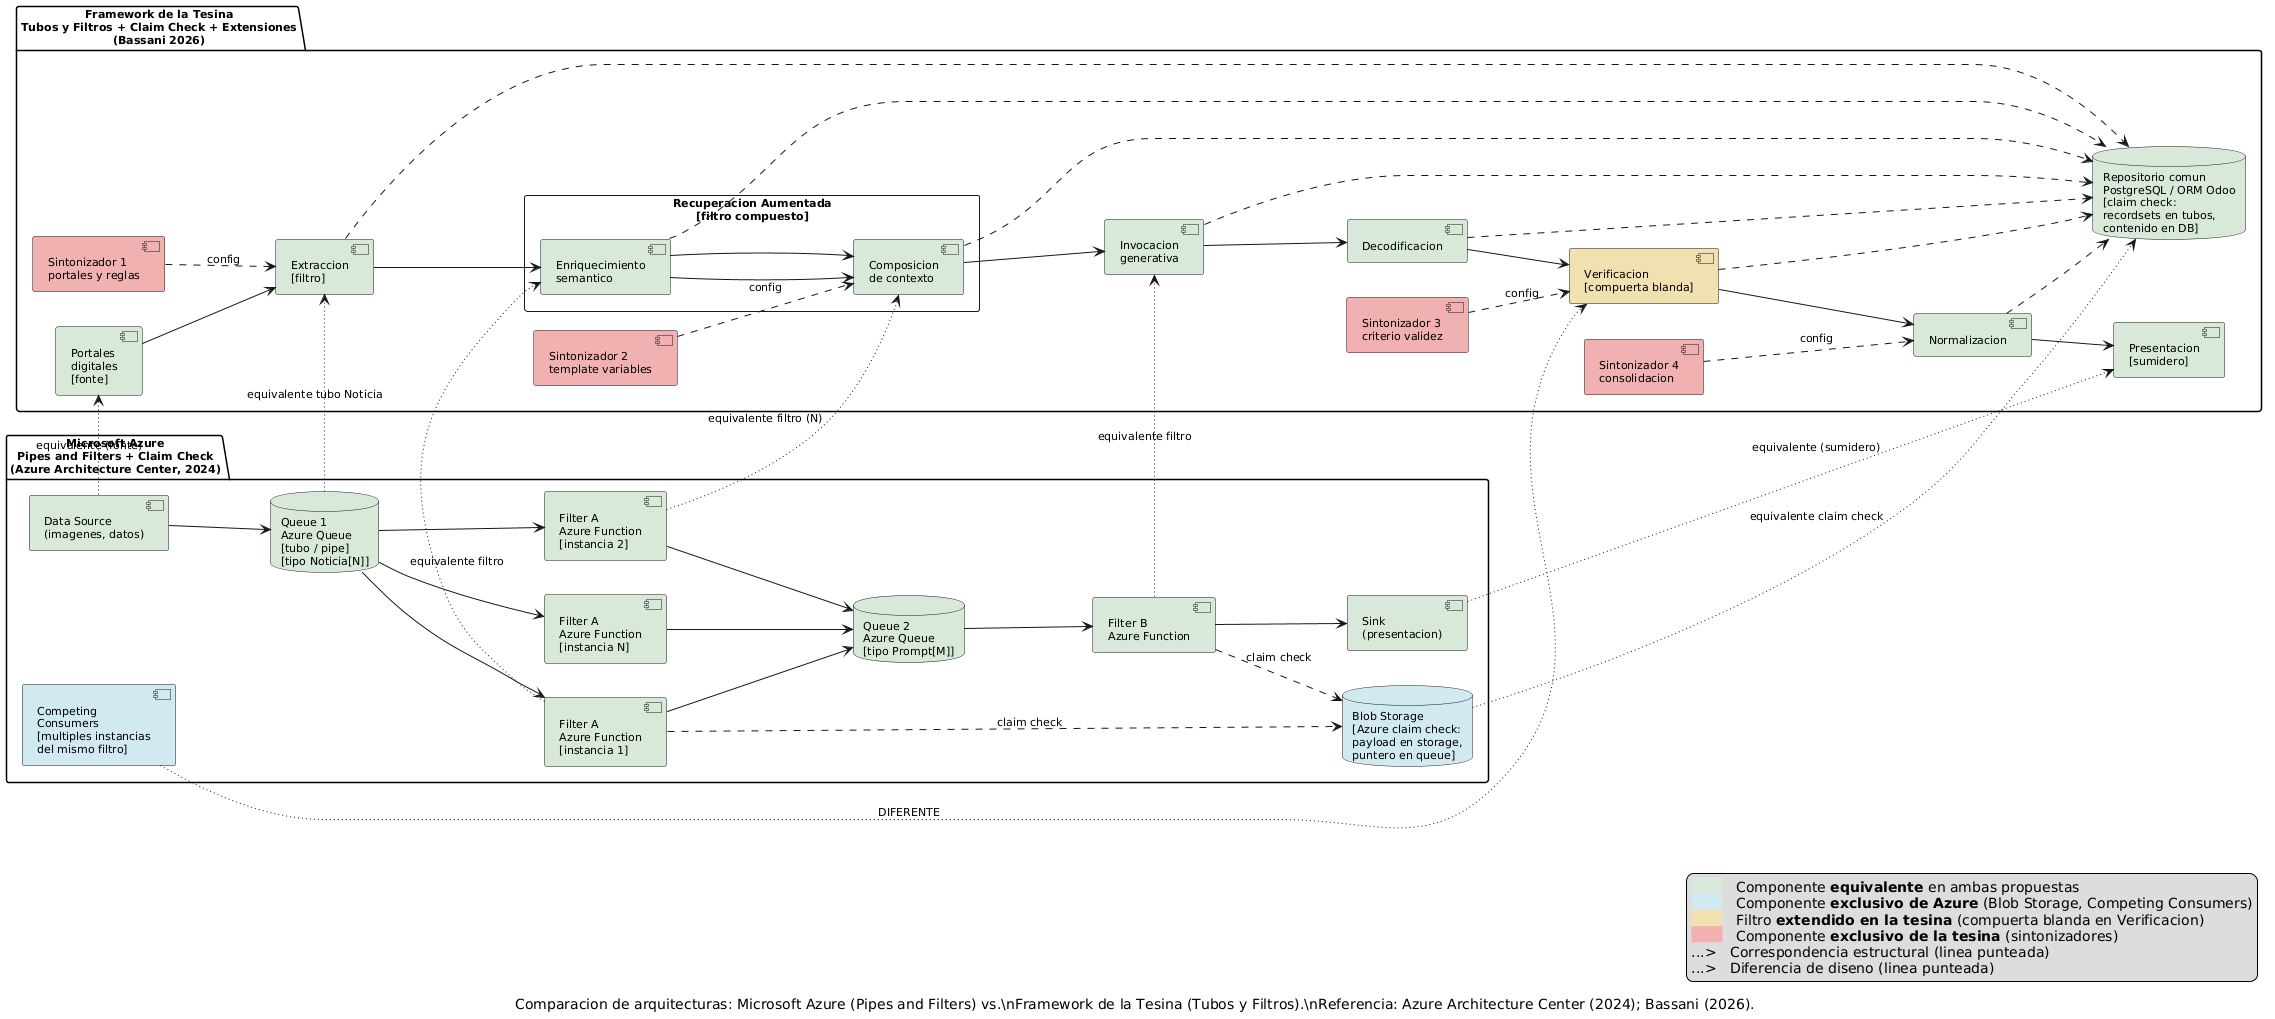
\includegraphics[width=\textwidth]{Diagrama-Comparativo.png}
  \caption{Comparación de arquitecturas: Microsoft Azure (Pipes and Filters
           con \textit{Claim Check} y \textit{Competing Consumers}) versus
           el framework propuesto en la presente tesina (Tubos y Filtros con
           \textit{Claim Check} sobre repositorio PostgreSQL y extensiones
           propias). La convención de colores indica componentes
           estructuralmente equivalentes (verde), exclusivos de cada
           propuesta (celeste para Azure, rosa para la tesina) y
           extendidos (amarillo: \textit{compuerta blanda} en
           Verificación). Las líneas punteadas marcan correspondencias
           entre componentes análogos.}
  \label{fig:arq-comparacion-azure}
\end{figure}

\subsubsection{Áreas de convergencia estructural}

La comparación revela coincidencias arquitectónicas directas en las cuatro
decisiones fundamentales del estilo:

\begin{itemize}
  \item \textbf{Separación de responsabilidades.} Ambas arquitecturas
        descomponen el procesamiento total en una cadena de filtros,
        cada uno responsable de una transformación específica.
        En Azure, cada \textit{Azure Function} encapsula una transformación
        (content moderation, resizing, etc.); en el framework de la tesina,
        cada filtro (Extracción, Enriquecimiento semántico, Composición de
        contexto, Invocación generativa, Decodificación, Verificación y
        Normalización) encapsula una transformación del pipeline.

  \item \textbf{Acoplamiento débil entre filtros.} En Azure, cada filtro
        (Azure Function) solo conoce su cola de entrada (Azure Queue) y
        su cola de salida; no conoce la identidad de otros filtros.
        El framework de la tesina aplica idéntica restricción como
        invariante~1 del estilo (Subsección~\ref{sec:arq-estilo-invariantes}):
        ningún filtro conoce la identidad ni la existencia de los demás.

  \item \textbf{Patrones de mensajería \textit{Claim Check}.} Azure documenta
        que las colas no transportan la carga útil completa sino punteros
        (claim checks) al Blob Storage, donde reside el contenido
        real~\citep{microsoft-azure:2024}. El framework de la tesina
        aplica exactamente el mismo principio sobre PostgreSQL vía el
        ORM de Odoo: los \textit{recordsets} transportan referencias por
        los tubos, mientras el contenido reside en el repositorio común
        (Subsección~\ref{sec:arq-car-repositorio}).

  \item \textbf{Composición libre según compatibilidad de schemas.}
        Azure permite reordenar y recombinar filtros siempre que los
        schemas de entrada y salida coincidan; el framework de la tesina
        habilita la misma flexibilidad mediante el cierre composicional
        del estilo Tubos y Filtros (Subsección~\ref{sec:arq-estilo-componentes})
        y los contratos de datos tipados del Apéndice~\ref{anexo:tipos}.
\end{itemize}

\begin{table}[H]
  \centering
  \caption{Correspondencia de componentes entre Azure y la presente tesis.}
  \label{tab:correspondencia-azure}
  \footnotesize
  \setlength{\tabcolsep}{4pt}
  \begin{tabularx}{\textwidth}{@{}l l l X@{}}
    \toprule
    \textbf{Rol} & \textbf{Microsoft Azure} & \textbf{Tesis} & \textbf{Mecanismo} \\
    \midrule
    Fuente & Data Source & Portales digitales & Flujo de entrada no tipado \\
    \addlinespace
    Tubo / pipe & Azure Queue Storage & Recordset Odoo (referencia) &
      Transporte unidireccional con contenido separado \\
    \addlinespace
    Filtro & Azure Function & Filtro del pipeline (Extracción, Enriquecimiento, \ldots) &
      Transformación local independiente \\
    \addlinespace
    Claim Check & Azure Blob Storage & Repositorio PostgreSQL / ORM Odoo &
      Contenido en almacén, referencia en queue \\
    \addlinespace
    Sumidero & Sink (presentación) & Capa de presentación (tableros, reportes) &
      Entrega al entorno externo \\
    \bottomrule
  \end{tabularx}
\end{table}

\subsubsection{Extensiones sobre el diseño de Microsoft}

El framework propuesto extiende la arquitectura de referencia de Microsoft
en cuatro dimensiones clave que responden a requerimientos específicos del
análisis de noticias con inteligencia artificial generativa:

\begin{enumerate}
  \item \textbf{Sintonizadores como deformación canónica del estilo.}
        Microsoft no documenta un mecanismo explícito para la configuración
        externa que no participe del flujo de datos. Los cuatro sintonizadores
        del framework (puertos, reglas de extracción, template de análisis,
        criterio de validez y política de consolidación) reifican la
        deformación canónica de los \textit{tuners} documentada por
        \citet[§3.13.2]{cristia:2025}. Esta decisión desacopla la intervención
        del experto del dominio del procesamiento del filtro, y preserva la
        pureza arquitectónica del estilo Tubos y Filtros: la configuración
        es un parámetro del filtro, no un dato que circule por la red de
        tubos.

  \item \textbf{Compuerta blanda en el filtro de Verificación.}
        Microsoft no aborda explícitamente cómo manejar la incertidumbre en
        la salida de los filtros. La arquitectura de la tesis introduce, en
        el filtro de Verificación, una \textit{compuerta blanda} que califica
        y marca los análisis no sustentados pero no los suprime: la decisión
        editorial última queda en manos del analista humano, no de un
        automatismo. Esta política responde a tres brechas identificadas en
        la revisión sistemática (Sección~\ref{sec:rsl-brechas}): la necesidad
        de evaluar la fidelidad del análisis a la evidencia empírica, de
        calibrar la incertidumbre de los scores y de habilitar procedimientos
        \textit{human-in-the-loop} de gobernanza editorial.

  \item \textbf{Cadena de procedencia como propiedad estructural.}
        Microsoft no documenta un mecanismo sistemático de trazabilidad
        documental de extremo a extremo. El framework de la tesis
        construye, como propiedad emergente del sistema de tipos, una cadena
        de procedencia continua que recorre el pipeline en sentido inverso:
        desde el \texttt{Resultado} final se puede reconstruir qué
        veredictos de verificación lo componen, sobre qué análisis se
        pronuncia cada uno, de qué respuestas crudas provienen, con qué
        \textit{prompts} ---y bajo qué \textit{template} y parámetros--- se
        generaron, sobre qué noticias se apoyó cada composición y de qué
        portal fue extraída cada noticia, cuándo y bajo qué reglas. Esta
        propiedad materializa, a nivel del dato, la auditabilidad lineal
        que motivó la elección del estilo (Subsección~\ref{sec:arq-estilo-justificacion})
        y resuelve la brecha de trazabilidad documental identificada por
        la revisión sistemática.

  \item \textbf{Agnosticidad del ejecutor de Verificación.}
        Microsoft no especifica quién ---o qué--- ejecuta la validación de
        los filtros. El framework de la tesis hace explícita la agnosticidad
        del ejecutor del filtro de Verificación: la decisión editorial ---o
        el procedimiento automático que la sustituye--- se incorpora como
        parámetro vía el sintonizador~3. En particular, cuando el ejecutor
        se apoya en agentes generativos que confrontan sus juicios ---caso
        documentado como \textit{LLM-as-a-judge} y verificación multiagente
        en la literatura contemporánea de agentes
        \citep{xi:2023}---, la sustituibilidad garantizada por las
        invariantes~1 y~2 habilita reemplazar el ejecutor sin alterar el
        resto del pipeline.
\end{enumerate}

\subsubsection{Diferencia significativa: escalabilidad horizontal versus agnosticidad del ejecutor}

Microsoft documenta el patrón hermano \textit{Competing Consumers}
\citep{microsoft-azure:2024} como mecanismo para escalar horizontalmente
filtros específicos: múltiples instancias del mismo filtro compiten por
los mensajes de una cola, distribuyendo la carga y mejorando el
\textit{throughput} en filtros \textit{bottleneck}. En el framework de la
tesis, la escalabilidad no se aborda mediante múltiples instancias del
mismo filtro ---aunque el diseño, por las invariantes~1 y~2, no la impide---
sino mediante la agnosticidad del ejecutor de Verificación: el ejecutor
puede ser un procedimiento automático, un revisor humano o un conjunto de
agentes confrontando sus juicios, según defina el sintonizador~3. Esta
decisión responde al mismo objetivo (gestionar la incertidumbre del
procesamiento generativo) por una vía distinta: en lugar de escalar
horizontalmente la verificación automática, el framework delega la decisión
final al experto del dominio, materializando la gobernanza editorial
\textit{human-in-the-loop} que la revisión sistemática identificó como
brecha crítica.

\subsubsection{Ventajas y compromisos comparados}

La comparación permite explicitar tres ventajas del diseño propuesto y
dos compromisos que acarrea:

\begin{itemize}
  \item \textbf{Ventaja --- control editorial explícito:} la compuerta
        blanda y la cadena de procedencia completa permiten al experto del
        dominio ejercer control sobre la calidad y fidelidad de los
        resultados, dimensión crítica en el análisis de noticias.
  \item \textbf{Ventaja --- configuración sin alterar el flujo:} los
        sintonizadores permiten parametrizar el comportamiento de los
        filtros sin inyectar datos en el pipeline, manteniendo la pureza
        arquitectónica del estilo.
  \item \textbf{Ventaja --- flexibilidad en la validación:} la
        agnosticidad del ejecutor de Verificación permite evolucionar
        desde validación manual a validación asistida por LLMs sin alterar
        la arquitectura base.
  \item \textbf{Compromiso --- menor escalabilidad horizontal inmediata:}
        la arquitectura de Azure, al documentar explícitamente
        \textit{Competing Consumers}, permite escalar filtros individuales
        de manera inmediata; el framework de la tesis podría adoptar el
        mismo patrón sin alterar el diseño, pero no lo prescribe en su
        configuración base.
  \item \textbf{Compromiso --- menor flexibilidad de recomposición:}
        Azure permite reordenar filtros libremente según compatibilidad
        de schemas; la tesis, al especializarse en el patrón de
        \textit{pipelines} (un único puerto de entrada y un único puerto
        de salida por filtro), restringe la recomposición a la sustitución
        y extensión por sintonizador, no al reordenamiento arbitrario
        (Subsección~\ref{sec:arq-car-especializaciones}). Este compromiso
        es deliberado, y responde a la naturaleza acíclica y lineal del
        análisis de noticias, donde las etapas deben ejecutarse en un
        orden fijo.
\end{itemize}

La Tabla~\ref{tab:comparacion-azure-diferencias} sintetiza las diferencias
de diseño y sus consecuencias prácticas.

\begin{table}[H]
  \centering
  \caption{Diferencias de diseño entre Azure y la presente tesis.}
  \label{tab:comparacion-azure-diferencias}
  \footnotesize
  \setlength{\tabcolsep}{4pt}
  \begin{tabularx}{\textwidth}{@{}l X X@{}}
    \toprule
    \textbf{Dimensión} & \textbf{Microsoft Azure} & \textbf{Tesis} \\
    \midrule
    Escalabilidad horizontal de filtros
      & \textit{Competing Consumers}: múltiples instancias del mismo filtro
        compiten por una cola.
      & No prescrita explícitamente; escalabilidad gestionada vía
        agnosticidad del ejecutor. \\
    \addlinespace
    Configuración de filtros
      & Externalizada (no detallada en el patrón).
      & Sintonizadores explícitos que NO participan del flujo de datos. \\
    \addlinespace
    Incertidumbre en la salida
      & No abordada explícitamente.
      & Compuerta blanda en Verificación con calibración de confianza. \\
    \addlinespace
    Trazabilidad documental
      & No explicitada como propiedad arquitectónica.
      & Cadena de procedencia como propiedad estructural del sistema de tipos. \\
    \addlinespace
    Flexibilidad de recomposición
      & Reordenamiento libre de filtros compatibles.
      & Restringida al patrón lineal + extensión por sintonizador. \\
    \bottomrule
  \end{tabularx}
\end{table}
